%%%%%%%%%%%%%%%%%%%%%%%%%%%%%%%%%%%%%%%%%%%%%%%%%%%%%%%%%%%%%%%%%%%%%%%%%%%%%
%
%  System        : 
%  Module        : 
%  Object Name   : $RCSfile$
%  Revision      : $Revision$
%  Date          : $Date$
%  Author        : $Author$
%  Created By    : Robert Heller
%  Created       : Mon May 13 10:52:26 2024
%  Last Modified : <240514.0847>
%
%  Description 
%
%  Notes
%
%  History
% 
%%%%%%%%%%%%%%%%%%%%%%%%%%%%%%%%%%%%%%%%%%%%%%%%%%%%%%%%%%%%%%%%%%%%%%%%%%%%%
%
%    Copyright (C) 2024  Robert Heller D/B/A Deepwoods Software
%			51 Locke Hill Road
%			Wendell, MA 01379-9728
%
%    This program is free software; you can redistribute it and/or modify
%    it under the terms of the GNU General Public License as published by
%    the Free Software Foundation; either version 2 of the License, or
%    (at your option) any later version.
%
%    This program is distributed in the hope that it will be useful,
%    but WITHOUT ANY WARRANTY; without even the implied warranty of
%    MERCHANTABILITY or FITNESS FOR A PARTICULAR PURPOSE.  See the
%    GNU General Public License for more details.
%
%    You should have received a copy of the GNU General Public License
%    along with this program; if not, write to the Free Software
%    Foundation, Inc., 675 Mass Ave, Cambridge, MA 02139, USA.
%
% 
%
%%%%%%%%%%%%%%%%%%%%%%%%%%%%%%%%%%%%%%%%%%%%%%%%%%%%%%%%%%%%%%%%%%%%%%%%%%%%%

\documentclass[12pt,twoside]{article}
\usepackage{graphicx}
\usepackage{mathptm}
\usepackage{times}
\usepackage{ifpdf}
\usepackage{footmisc}
\ifpdf
\usepackage[pdftex,
            pagebackref=true,
            colorlinks=true,
            linkcolor=blue,
            unicode
           ]{hyperref}
\else
\usepackage[ps2pdf,
            pagebackref=true,
            colorlinks=true,
            linkcolor=blue,
            unicode
           ]{hyperref}
\usepackage{pspicture}
\fi
\usepackage{url}
\pagestyle{headings}
\emergencystretch=50pt
\setcounter{tocdepth}{3}
\setcounter{secnumdepth}{3}
\title{''Bates Motel'' Lighted Building Sign Board Instructions}
\author{Robert Heller \\ The Country Robot \\ Wendell, MA, USA}
\date{\today}
\begin{document}
\maketitle

\begin{centering}%
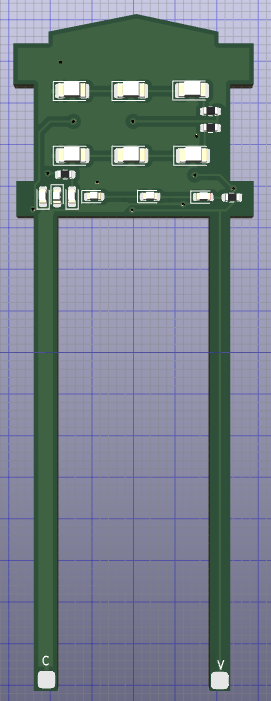
\includegraphics[height=4in]{BatesMotelFrontPCB.png}%
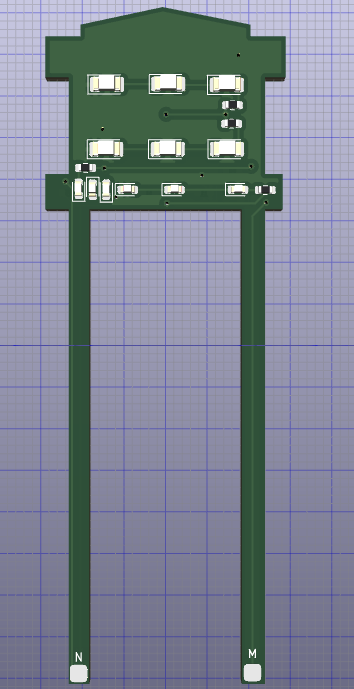
\includegraphics[height=4in]{BatesMotelBackPCB.png}\\
{\Large Front~~~~~~~~~~~~~~~~~~~~~Back}\\
\end{centering}

This is a printed circuit board containing SMD LEDs meant to replace the
static sign in the Perplexing Puzzles Plus HO Scale Roadside Motel (Bates
Motel) Kit\footnote{Available on E-Bay at
\url{https://www.ebay.com/itm/254591118293}.}. This PCB has three sets of LEDs
to light up three separate sections of the sign, the main name part (''Bates
Motel''), the word ``No'' and the word ``Vacancy'', on both sides of the sign.
It is a common cathode and includes resistors for 12VDC operation, either
staticly or with some sort of lighting effects electronics.

There are four solder pads at the bottom of the support posts, labeled: C
(common, +), V (''Vacency'', -), M (Main: ``Bates Motel'', -), and N (''No'',
-).

\end{document}
